\documentclass{beamer}
\beamertemplatenavigationsymbolsempty
\usecolortheme{beaver}
\setbeamertemplate{blocks}[rounded=true, shadow=true]
\setbeamertemplate{footline}[page number]

\usepackage[utf8]{inputenc}
\usepackage[english]{babel}
\usepackage{amssymb,amsfonts,amsmath,mathtext}

\usepackage{booktabs} 
\usepackage{epigraph}
\usepackage{csquotes}
\usepackage{blindtext}
\usepackage[outline]{contour}
\usepackage[figuresleft]{rotating}
\usepackage{tabularx}
\usepackage{varwidth}


\usepackage[all]{xy} 
\usepackage{array}
\usepackage{multicol}
\usepackage{hyperref}
\usepackage{subcaption}

\graphicspath{{../figures/}{../code/notebooks/pic}  }

%----------------------------------------------------------------------------------------------------------
\title[\hbox to 56mm{Online expert aggregation}]{Influence of hyperparameters on online aggregation with countable experts}
\author[N.\,P.~Ivkin]{Sergey Kunin-Bogoiavlenskii}
\institute[MIPT] % Your institution as it will appear on the bottom of every slide, may be shorthand to save space
{
Moscow Institute of Physics and Technology \\ % Your institution for the title page
\medskip
\textit{kunin-bogoiavlenskii.sm@phystech.edu} % Your email address
\par\smallskip\emph{Expert:} R.\,D.~Zukhba
\par\smallskip\emph{Consultant:} A.\,V.~Zukhba
}


%\institute{Moscow Institute of Physics and Technology}
%\date{\footnotesize
%%\par\smallskip\emph{Course:} My first scientific paper\par (Strijov's practice)/Group 125 
%\par\smallskip\emph{Expert:} R.\,D.~Zukhba
%\par\smallskip\emph{Consultant:} A.\,V.~Zukhba}
%\par\bigskip\small 2024}
\date{\today}

%----------------------------------------------------------------------------------------------------------
\begin{document}
%----------------------------------------------------------------------------------------------------------
\begin{frame}
\thispagestyle{empty}
\maketitle
\end{frame}

%-----------------------------------------------------------------------------------------------------
%\begin{frame}{Goal of research}
%..
%\end{frame}
%-----------------------------------------------------------------------------------------------------


\begin{frame}
\frametitle{What can be forecast?}
%\begin{displayquote}
%There are two kinds of forecasters: those who \\ don’t know, and those who don’t know they don’t know. \\ John Kenneth Galbraith
%\end{displayquote}
\setlength{\epigraphwidth}{0.45\textwidth}

\epigraph{Tell us what the future holds, so we may know that you are gods.}{\textit{Isaiah 41:23}}
%
%\epigraph{There are two kinds of forecasters: those who \\ don’t know, and those who don’t know they don’t know.}{\textit{John Kenneth Galbraith}}
%\blindtext
\begin{itemize}
\item Weather conditions
\item Economic trends
\item Technology advancements
\item Consumer behavior
\item Population growth
\item Political elections outcomes

\end{itemize}
\end{frame}


%------------------------------------------------
\subsection{Goal of research} 

\begin{frame}
\frametitle{Goal of research}
\setlength\epigraphwidth{.45\textwidth}
\epigraph{Prediction is very difficult, especially if it's about the future.}{\textit{Niels Bohr}}
%\blindtext

\begin{block}{Goal}
Examining the influence of hyperparameters on the performance of the aggregation algorithm with a countable number of experts
\end{block}


\begin{block}{Targets}
\begin{enumerate}
\item Time series generator implementation
\item Aggregating algorithm implementation
\item Experiments with various hyperparameters    
\end{enumerate}
\end{block}

%\begin{enumerate}
%\item Time series generator implementation
%\item Aggregating algorithm implementation
%\item Experiments with various hyperparameters    
%\end{enumerate}


\end{frame}
%-----------------------------------------------------------------------------------------------------

\begin{frame}{Literature}
    \begin{itemize}
    \item V.\,V’yugin, V.\,Trunov. 2023. Prediction of Locally Stationary Data Using Prediction with
Expert Advice. \url{http://www.jip.ru/2023/470-487-2023.pdf}
     \item O.\,Bousquet, M.\,Warmuth. 2002. \url{https://www.jmlr.org/papers/volume3/bousquet02b/bousquet02b.pdf}

    
    \item N.\,Cesa-Bianchi, G.\,Lugosi. 2006. \\
    Prediction, Learning, and Games.
    \url{https://ii.uni.wroc.pl/~lukstafi/pmwiki/uploads/AGT/Prediction_Learning_and_Games.pdf}.
    
    \item Hyndman,\,R.\,J. \& Athanasopoulos,\,G., 2nd edition. 2018. Forecasting: Principles and Practice. \url{https://otexts.com/fpp2/}
    
   %
%    \item Miles Cranmer, Sam Greydanus, Stephan Hoyer, Peter Battaglia, David Spergel, and Shirley Ho. Lagrangian neural networks. arXiv preprint arXiv:2003.04630, 2020.
%
%    \item Обработка датасета PAMAP2. https://github.com/andreasKyratzis/PAMAP2-Physical-Activity-Monitoring-Data-Analysis- and-ML/blob/master/pamap2.ipynb
  
    \end{itemize}
\end{frame}

%------------------------------------------------
\section{Problem statement} 
\subsection{Data} 

\begin{frame}
\frametitle{Problem statement}

\epigraph{There are two kinds of forecasters: those who \\ don’t know, and those who don’t know they don’t know.}{\textit{John Kenneth Galbraith}}

\textbf{Data}

It is assumed that there are multiple generators, whose structure is unknown to the predictors. 
The time series is obtained by merging segments, each produced by one of the generators. 
These segments are called areas of stationarity, and can be studied using machine learning methods. 

\bigskip
\textbf{Gerators implemented:}
\begin{itemize}
\item Linear 
\item ARMA
\end{itemize}




\end{frame}

%------------------------------------------------

\subsection{Terms} 

\begin{frame}
\frametitle{Problem statement}

\textbf{Terms}
\begin{itemize}
\item $X$ --- signals space
\item $Y$ --- responses space
\item $\mathcal{N}$ --- set of experts, indexed by natural numbers \\
\item $\mathsf{D}$ --- desicion space, to which predictions belong \\
\item $\lambda: \mathsf{D} \times \mathsf{Y} \rightarrow \mathbb{R}_+$ --- nonnegative loss function \\

\item $L^i_T = \sum\limits_{t = 1}^T l^i_t$ --- cumulative loss of expert $i$ during the first T steps \\
\item $H_T = \sum\limits_{t = 1}^T h_t$ --- master's cumulative loss during the first T steps \\
%\item $R^i_T = H_T - L^i_T$ --- master's regret relative to the expert $i$ \\
\item $R_T= H_T - L_T$ --- master's regret relative to the best partition, where $L_T$ is the cumulative loss of the best partition. 
\end{itemize}


\end{frame}

%------------------------------------------------

\setbeamertemplate{enumerate items}[default]
\subsection{Algorithm} 
\begin{frame}
\frametitle{Problem statement}

\textbf{Algorithm}

\bigskip
%
%\begin{enumerate}%[label={(\arabic*)}]
%\item Expert initialization
%\item Predictions
%\item Loss weights update
%\item Mixing weights update
%\end{enumerate}
FOR $t = 1, 2, \dots$:
\begin{enumerate}
\item Expert $f^t$ initialization
\item Experts' predictions $f_t^i = f_t^i(x_t),\ 1 \le i \le t$ 
\item Master's prediction evaluation $\gamma_t = \mathsf{Subst}(\mathbf{f_t}, \mathbf{\widehat{w}_t})$
\item Computation of master's loss $h_t = \lambda(p_t, y_t) $ and experts' losses $l_t^i$ 
%\item Modify experts' weights in two steps:

\item \textbf{Loss Update} weights modification
\item \textbf{Mixing Update} weights modification

\end{enumerate}

ENDFOR

\end{frame}


%------------------------------------------------
\section{Experiments} 
%\subsection{Hyperparameters} 

\begin{frame}
\frametitle{Experiments}

\textbf{Metric --- $R_T$,  the regret}
\begin{block}{Initialization weights}
Default weights: $w_1^i = \frac{1}{(i+1)\ln^2(i+1)}$

Experimental:  $\frac{1}{i^\alpha}$, $\frac1c$,  $\frac{1}{(i+4)\ln(i+4)\ln^2\ln(i+4)}$, etc.
\end{block}

\begin{block}{Noise}
Different noise variance leads to diverse ability of experts to train, which opens curious quialities of the master algorithm
\end{block}

\begin{block}{Window size}
As the algorithm does not know the locations of generator switches, finding an optimal training window is also a challenge.
\end{block}

\end{frame}

%------------------------------------------------

\begin{frame}
\frametitle{Experiments}

\begin{block}{Mixing update scheme}
$ \widetilde{w}_{t+1}^i = \sum_{q=1}^t\beta_t(q)\widetilde{w}_q^i  $
\begin{itemize}
\item Start Vector Share - default scheme in GMPP
\item Uniform Past Share
\item Decaying Past Share
\item Increasing Past Share - new proposed scheme:

 \[\beta_t(q) =
    \begin{cases}
    \alpha_t(t-q)^\gamma\frac{1}{Z_t}, & 1 \le q < t \\
    1 - \alpha_t, & q = t
    \end{cases}\]
    \hfill ,with $Z_t = \sum_{q=1}^{t-1}(t-q)^\gamma, \gamma > 0$. 
\end{itemize}


\end{block}

\begin{block}{Mixing update coefficients}
Default coefficient: $\alpha_t = \frac{1}{t+1}$

Experimental:  $\frac{1}{(t+1)^\beta}$, $\frac{1}{c}$, $\frac{1}{(t+c)}$, $\frac{1}{e^{t/3}}$, etc.

\end{block}

\end{frame}

%------------------------------------------------



%\begin{frame}
%\frametitle{Loss plot}
%
%\subsection{Influence of Noise}
%\begin{figure}[htb]
%    \centering % <-- added
%\begin{subfigure}{0.36\textwidth}
%  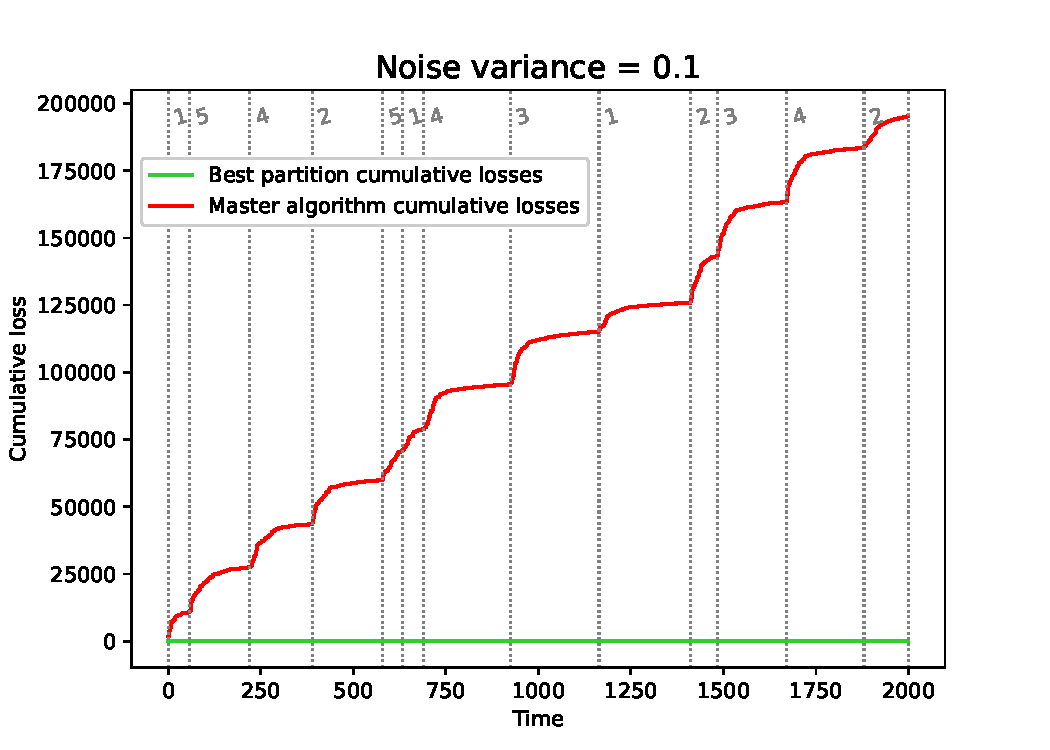
\includegraphics[width=\linewidth]{noise_0.1}
%  \caption{$\sigma^2$ = 0.1}
%  \label{fig:n_1}
%\end{subfigure}\hfil % <-- added
%\begin{subfigure}{0.36\textwidth}
%  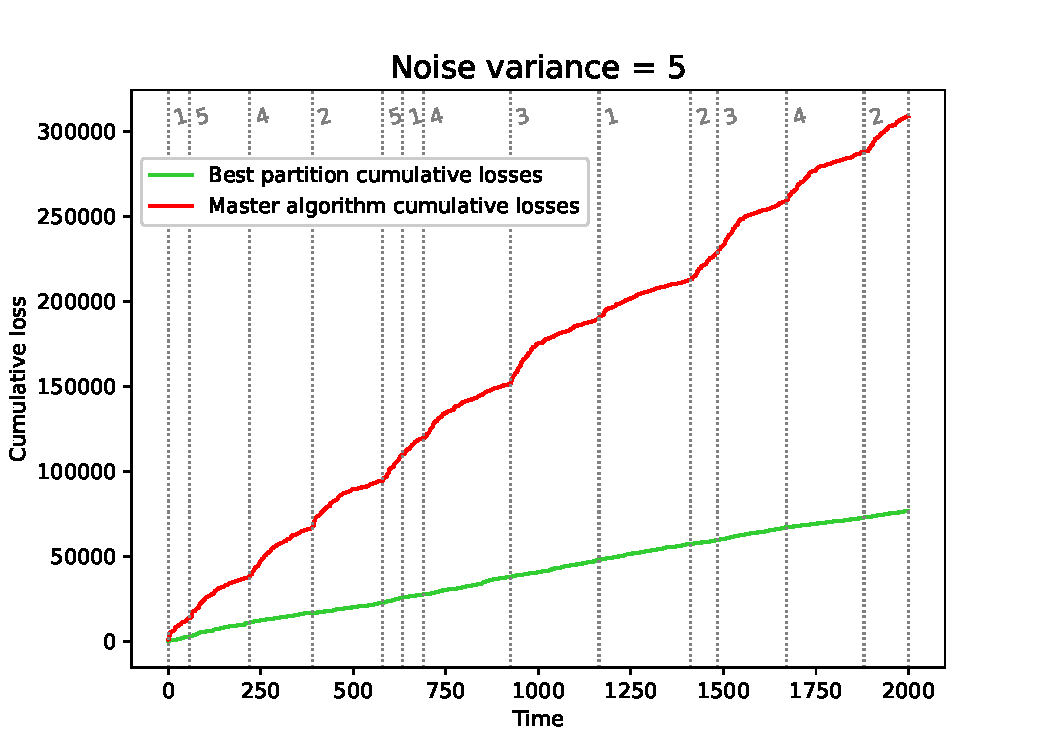
\includegraphics[width=\linewidth]{noise_5}
%  \caption{$\sigma^2$ = 5}
%  \label{fig:n_5}
%\end{subfigure}
%
%\medskip
%\begin{subfigure}{0.36\textwidth}
%  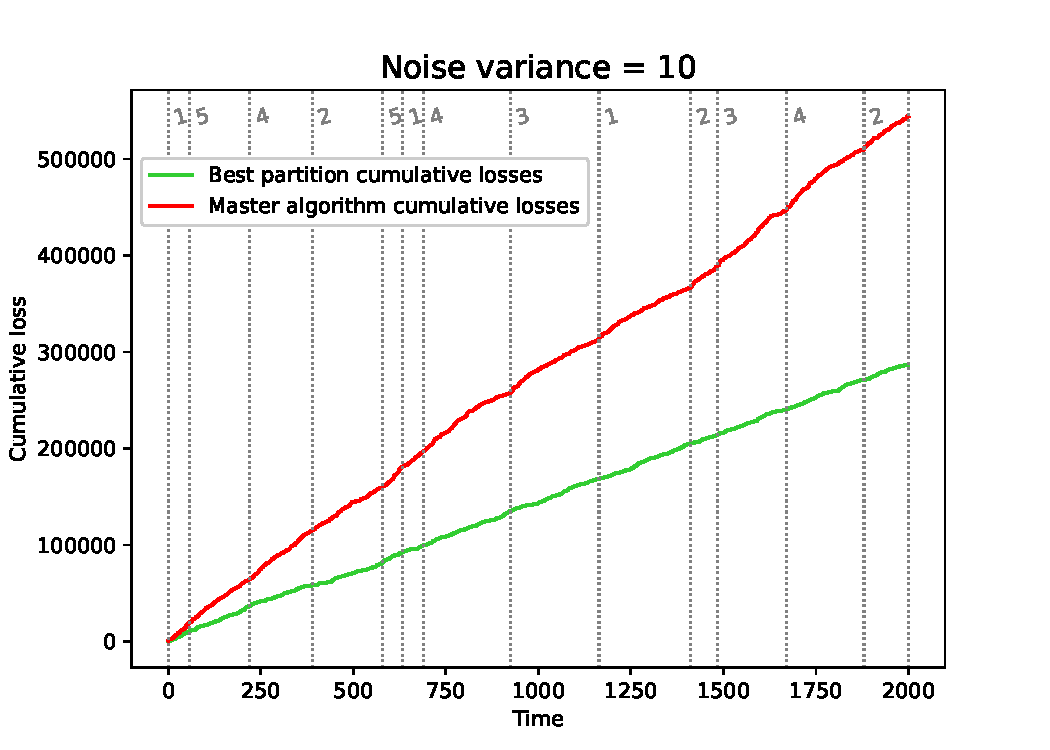
\includegraphics[width=\linewidth]{noise_10}
%  \caption{$\sigma^2$ = 10}
%  \label{fig:n_10}
%\end{subfigure}\hfil % <-- added
%\begin{subfigure}{0.36\textwidth}
%  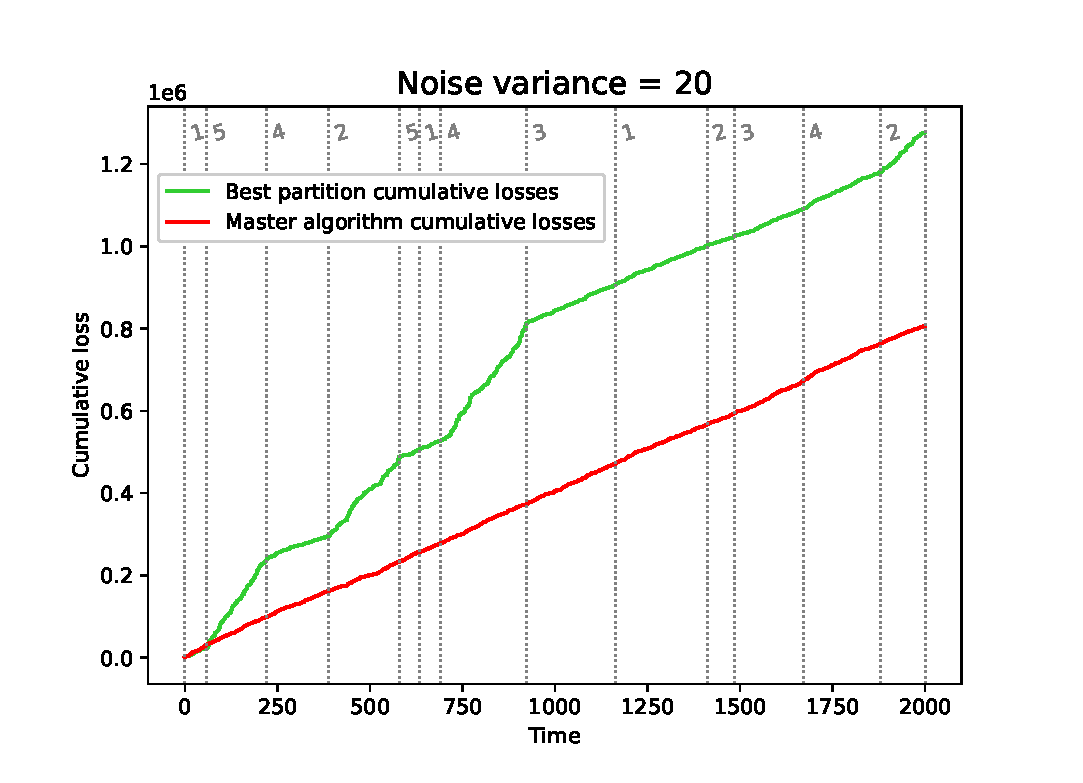
\includegraphics[width=\linewidth]{noise_20}
%  \caption{$\sigma^2$ = 20}
%  \label{fig:n_20}
%\end{subfigure}
%
%\caption{\begin{varwidth}[t]{\linewidth}\centering Total losses with different noise variance $\sigma^2$  \\ (alpha function is defaut, weight function is default, window size = 10)\end{varwidth}}
%
%%\caption{Total losses for different noise variance $\sigma^2$}
%\label{fig:noises}
%\end{figure}
%
%
%\end{frame}
%
%%------------------------------------------------

\begin{frame}
\frametitle{Initialization weights}
\begin{figure}[htb]
\centering % <-- added
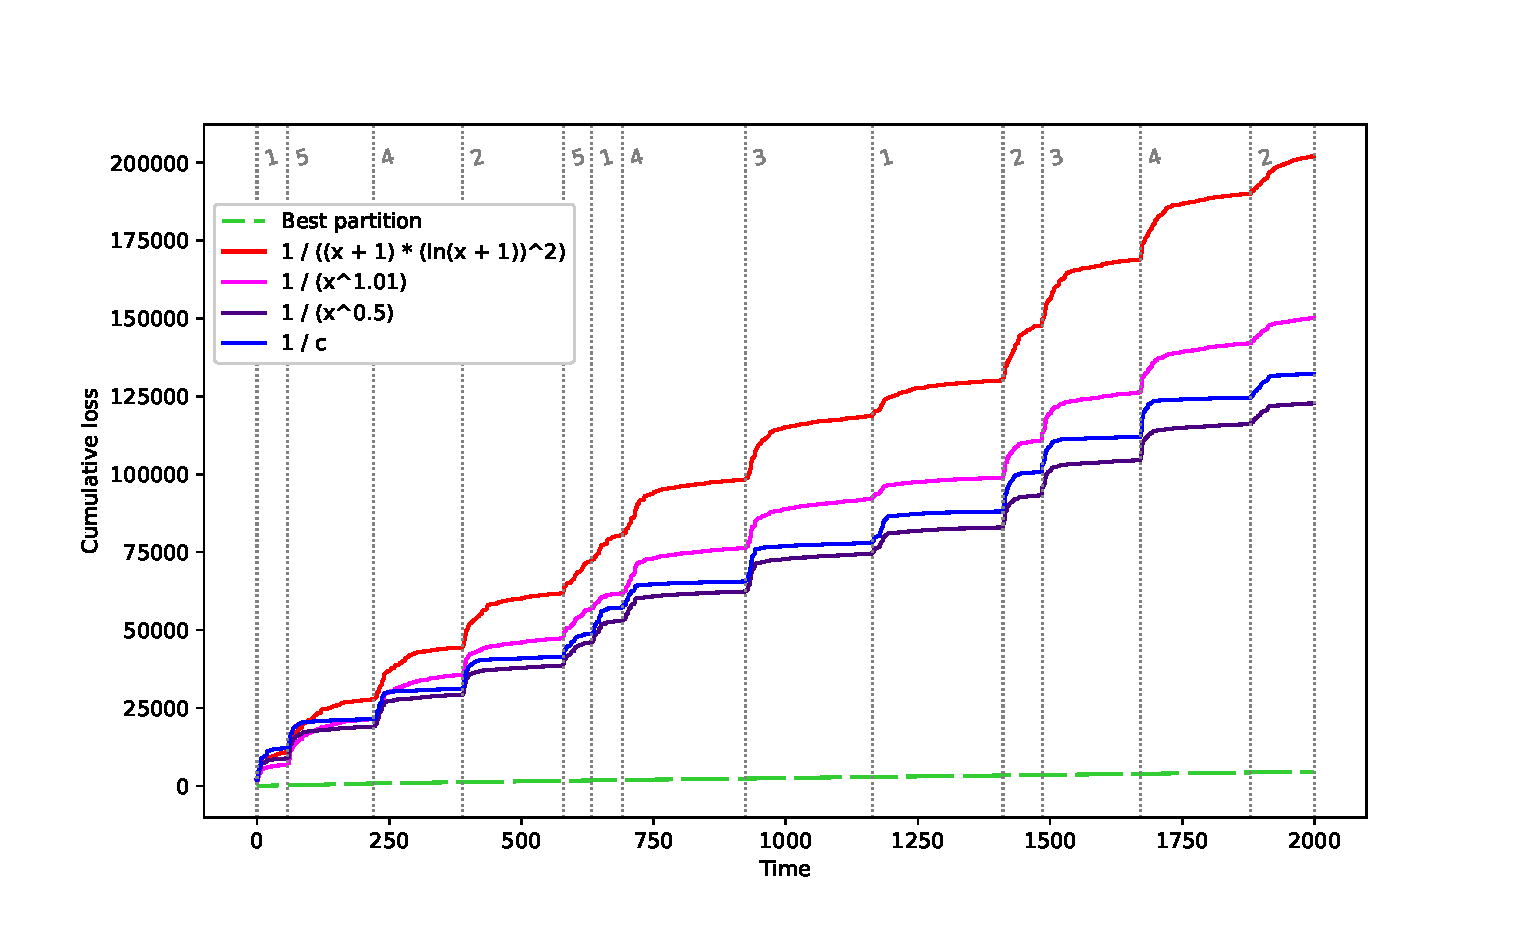
\includegraphics[width=1\linewidth]{diff_wf}
%\caption{Total loss for different weight functions}
\caption{\begin{varwidth}[t]{\linewidth}\centering Total loss for different weight functions \\(alpha function is defaut, $\sigma^2 =1$, window size = 10)\end{varwidth}}


\end{figure}

\end{frame}

%------------------------------------------------
\begin{frame}


\frametitle{Noise}

\begin{table}[H]
\centering
%\caption{Regret for different Mixing Update schemes and Noise}
\caption{\begin{varwidth}[t]{\linewidth}\centering Regret with different Mixing Update schemes and Noise Variance \\ (alpha function is defaut, weight function is $1/x^{1.01}$, window size = 10)\end{varwidth}}
\label{tab:alpha}
\begin{tabular}{c|cccc}
\toprule
& \multicolumn{3}{c}{Mixing scheme} \\
\toprule
{Noise variance} & \centering increasing past & \centering start & \centering uniform past &  \\
\midrule
0.10 & 114564.74 & 131578.01 & 115927.25 \\
1 & 110438.09 & 132268.30 & 110569.83 \\
2 & 105398.29 & 136043.26 & 103136.06 \\
5 & 92343.75 & 144554.62 & 83630.45 \\
6 & 89032.63 & 146382.86 & 25178.60 \\
7 & 29417.82 & 144827.02 & -9208.74 \\
8 & -13307.43 & 147510.57 & -55905.83 \\
%9 & -66578.18 & 111455.10 & -79922.70 \\
10 & -120166.34 & 90089.56 & -377184.32 \\
%11 & -553834.55 & -4217467.46 & -4977614.29 \\
12 & -1123130.94 & -420588.94 & -1354731.42 \\
%13 & -1127803.13 & -184977.56 & -1365609.14 \\
%14 & -1265872.25 & -213233.53 & -1633244.28 \\
15 & -1508510.73 & -1205600.59 & -1862352.43 \\
%20 & -9004436.41 & -8784588.25 & -9007978.86 \\
%50 & -14242897.85 & -4704221.50 & -14879230.26 \\
\bottomrule
\end{tabular}
\end{table}


\end{frame}

%------------------------------------------------
\begin{frame}
\frametitle{Mixing schemes}
\begin{figure}[htb]
\centering % <-- added
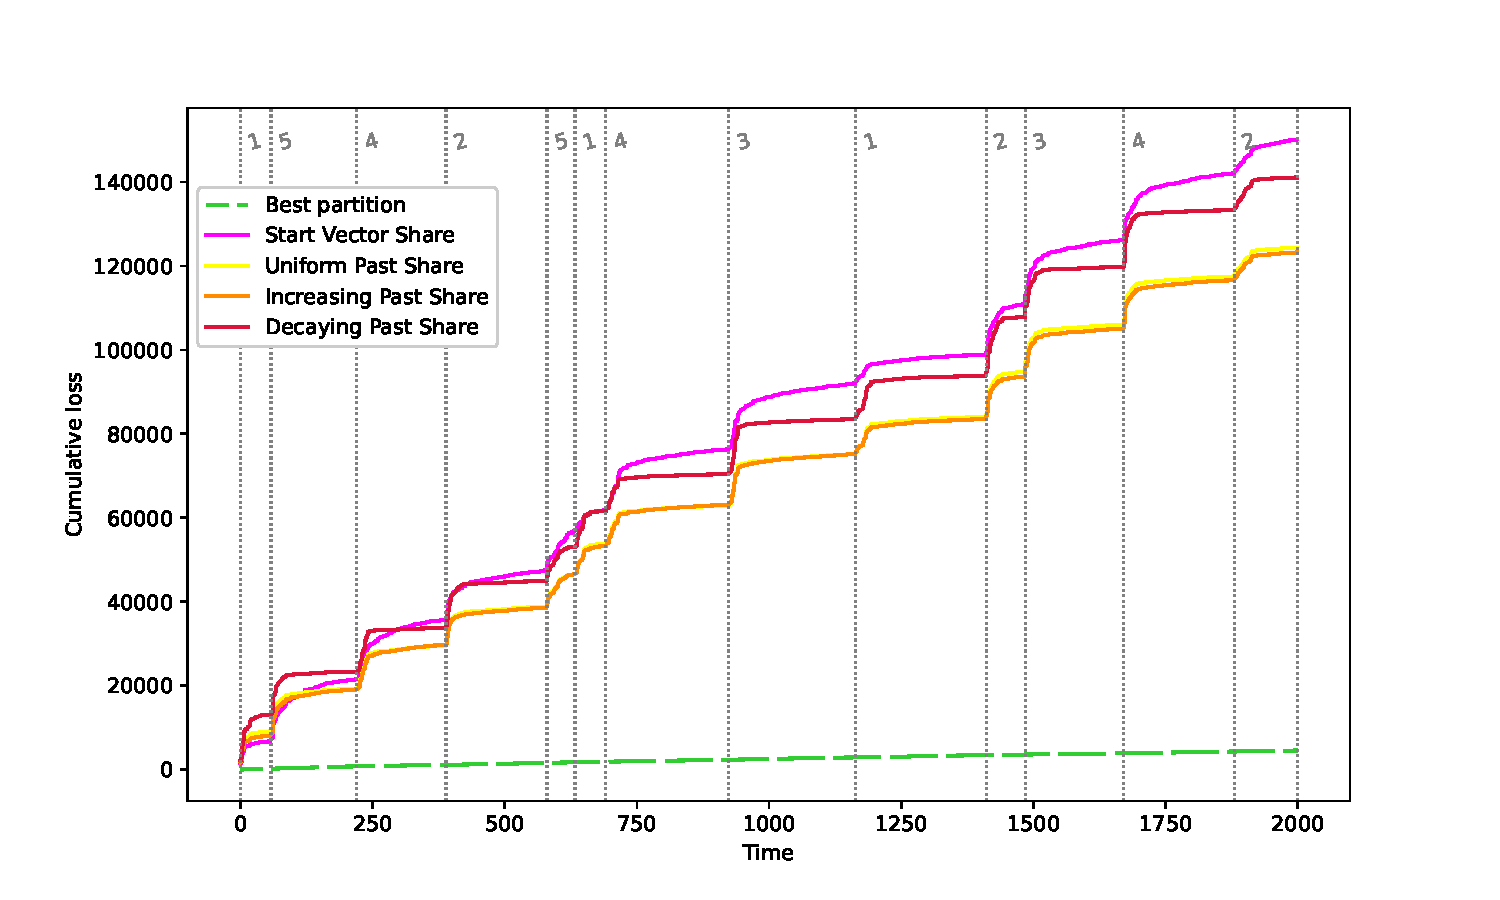
\includegraphics[width=1\linewidth]{diff_mt}
\caption{\begin{varwidth}[t]{\linewidth}\centering Total loss with different mixing schemes  \\ (default alpha function, weight function is $1/x^{1.01}$, window size = 10)\end{varwidth}}
%\caption{Total loss for different mixing schemes}
\medskip
\end{figure}


\end{frame}

%------------------------------------------------

%\begin{frame}
%
%
%\frametitle{Alpha coefficients}
%\begin{table}[H]
%\centering
%%\caption{Regret with different Alpha and Weight Functions in Start Vector Share Update scheme}
%\caption{\begin{varwidth}[t]{\linewidth}\centering Regret with different Alpha and Weight Functions in Start Vector Share Update scheme  \\($\sigma^2 =1$, window size = 10)\end{varwidth}}
%\begin{tabular}{r|ccc}
%\toprule
% & \multicolumn{3}{c}{Weight function} \\
%\toprule
%{Alpha function} &
%\centering $\dfrac{1}{{(x+1)\ln^2(x+1)}}$ &
%\centering $\dfrac{1}{x^{1.01}}$ &
%\centering $\dfrac{1}{x^{0.5}}$ 
%\tabularnewline
%\midrule
%$1 / (t + 1)$ & 175594.64 & 132268.30 & \contour{black}{108630.68} \\
%$1 / (t + 1)^{0.5}$ & 245494.10 & 207099.32 & 164079.31 \\
%$1 / (t + 1)^{1.5}$ & 130339.21 & 125699.71 & 130185.66 \\
%$1 / (t + 1)^2$ & 136029.09 & 134929.54 & 133876.06 \\
%$1 / e^{t/3}$ & 136413.87 & 135409.06 & 134012.15 \\
%$1 / (t + 10)$ & 175411.17 & 132208.09 & \contour{black}{108638.55} \\
%$1 / (t + 100)$ & 173760.98 & 131623.56 & \contour{black}{108732.56}\\
%$1 / (t + 1000)$ & 162129.20 & 127165.47 & 110389.16 \\
%%$1 / 100$ & 220008.81 & 163117.40 & 129035.87 \\
%%$1 / 500$ & 198094.83 & 141385.79 & 111706.58 \\
%%$1 / 1000$ & 184324.73 & 135612.25 & \contour{black}{109449.15} \\
%%$1 / 5000$ & 147561.46 & 121905.50 & 115147.43 \\
%%$1 / 10000$ & 136414.42 & 119357.81 & 120634.74 \\
%%$1 / 50000$ & 130783.65 & 125141.06 & 129963.25 \\
%\bottomrule
%\end{tabular}
%\end{table}
%\end{frame}

%------------------------------------------------


\begin{frame}
\frametitle{Conclusion}

\begin{block}
    
    Summary
        
    \begin{itemize}
  
        \item Generators and algorithm implemented
        \item Correctness of the algorithm veryfied
        \item A series of experiments conducted
        \item Enhanced weight functions achieved
        \item New Mixing Update Scheme proposed

    \end{itemize}
    \end{block}    
    
    \begin{block}
    
    Further directions of work
    
    \begin{itemize}
    	\item Experiment with time series of other order of length.      
	\item Run experiments on real data.
        \item Theoretically prove that the obtained functions are better.             
    \end{itemize}
    \end{block}

    
\end{frame}


\begin{frame}
\Huge{\centerline{The End}}
\end{frame}

\end{document} 